% !TeX spellcheck = sk_SK
\chapter{Analýza dynamiky balansujúceho robota}
\label{ch:analyza}

Dvojkolesový robot predstavuje z mechanického uhla pohľadu sústavu podobnú prevrátenému kyvadlu – teda sústavu, ktorá je inherentne nestabilná, a teda vyžaduje implementáciu robustného regulátora. Aby bol tento návrh možný, potrebujeme vytvoriť matematický model tohto systému, ktorý nám umožní navrhúť optimálny regulátor. Po zvážení sme usúdili, že bude výhodné takýto model vytvoriť osobitne pre časť podvozku s kolesami a pre šasi robota, ktoré tvorí prevrátené kyvadlo a tieto následne skombinovať.
Pracovať budeme s modelom navrhnutým Rich Chi Ooi \cite{Oochi2003} a mierne upraveným v práci\cite{TWIP}.

\section{Model kolesa}

Matematický model správania sa kolesa nebudeme odvádzať pre každé koleso zvlášť, ale budeme predpokladať, že obe kolesá sú identické, a teda aj rovnice budú pre obe rovnaké.
\begin{figure}
\centering
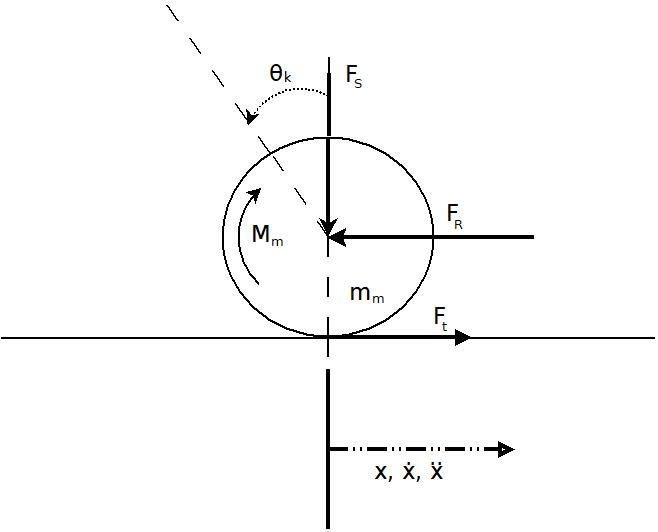
\includegraphics[width=10cm]{wheelForces}
\caption{Model kolesa}
\label{fig:wheelForces}
\end{figure}

\figurename~\ref{fig:wheelForces} znázorňuje koleso robota aj so všetkými silami, ktoré naň pôsobia, pričom:

\begin{multicols}{2}
\begin{itemize}
\item $\theta$ = uhol náklonu šasi
\item $m_k$ = hmotnosť kolesa 
\item $F_s$ = sila, ktorou na koleso pôsobí šasi
\item $F_R$ = reakčná sila medzi kolesom a šasi
\item $F_t$ = trecia sila medzi zemou a kolesom
\item $J_k$ = zotrvačnosť kolesa
\item $r$ = polomer kolesa 
\item $M_m$ = točivý moment
\item $x$ = poloha v x-ovej osi
\end{itemize}
\end{multicols}

V rovniciach budeme ďalej predpokladať, že robot sa nepohybuje do strán, ale len vpred alebo vzad. Do úvahy budeme musieť ale vziať to, že robot bude pri pohybe ovplyvňovaný vonkajšími stimulmi aj samotným momentom motora. Na začiatok využitím Newtonovho zákona pohybu v X-ovej osi odvodíme:
\begin{equation}
\begin{gathered}
\sum{F_x} = ma \\
m_k \ddot{x} = F_t - F_R
\end{gathered}
\label{eq:forceOnWheeles}
\end{equation}
A potom vyjadríme súčet momentov okolo stredu kolesa:
\begin{equation}
\begin{gathered}
\sum{M} = J \alpha \\
J_k\ddot{\theta} = M - F_f r
\end{gathered}
\label{eq:zotrvacnost}
\end{equation}

Ak teda vyjadríme točivý moment DC motora ako rozdiel zotrvačnosti motora vynásobeného okamžitým uhlovým zrýchlením a momentu záťaže, môžeme pokračovať v odvodzovaní:
\begin{equation}
\begin{gathered}
M_m = J \dfrac{d \mathrm{\omega}}{d \mathrm{t}} - M_Z
\\
M = M_m - M_Z = \dfrac{-K_M K_e}{R} \dot{\theta}+ \dfrac{K_M}{R} V_m
\end{gathered}
\label{eq:moment}
\end{equation}

kde:
$\quad K_Z$ = moment záťaže

$\quad K_M$ = momentová konštanta

$\quad K_e$ = elektrická konštanta motora

$\quad R$ = odpor vinutia motora

$\quad U_m$ = el. napätie na motore

Konštanty $K_M$, $K_e$ je možné získať zo vzťahov \eqref{eq:motoroveKonstanty}:
\begin{equation}
K_e = \dfrac{U_X}{\omega} \quad \quad K_M = \dfrac{F_X r}{I_X}
\label{eq:motoroveKonstanty}
\end{equation}


Dosadením do \eqref{eq:zotrvacnost} z \eqref{eq:moment} tak získame:
\begin{equation}
F_f = \dfrac{-K_M K_e}{Rr}\dot{\theta}_k + \dfrac{K_M}{Rr}U_m - \dfrac{K_k}{r}\ddot{\theta}_k
\end{equation}
Túto rovnicu je možné prepísať pomocoou \eqref{eq:forceOnWheeles} a nájsť tak rovnicu pre jedno koleso:
\begin{equation}
\begin{gathered}
m_m \ddot{x} = F_f - F_R =  \dfrac{-K_m K_e}{Rr}\dot{\theta}_k + \dfrac{K_M}{Rr}U_m - \dfrac{J_k}{r}\ddot{\theta}_k - F_R \\
\downdownarrows
\\
\theta = \dfrac{x}{r}
\\
\downdownarrows
\\
m_m \ddot{x} = F_f - F_R = \dfrac{-K_M K_e}{R r^2}\dot{x}_k + \dfrac{K_M}{Rr}U_m - \dfrac{J_k}{r^2}\ddot{x}_k - F_R
\end{gathered}
\end{equation}

Vynásobením dvoma (dve kolesá) získavame kompletný model podvozku:
\begin{equation}
\begin{gathered}
2m_m \ddot{x} = 2F_f - 2F_R = \dfrac{-2K_M K_e}{R r^2}\dot{x}_k + \dfrac{2K_M}{Rr}U_m - \dfrac{2J_k}{r^2}\ddot{x}_k - 2F_R
\\
2(m_m - \dfrac{2J_k}{r^2}) \ddot{x} = \dfrac{-2K_M K_e}{R r^2}\dot{x}_k + \dfrac{2K_M}{Rr}U_m - 2F_R
\end{gathered}
\label{eq:wheels}
\end{equation}
\newpage
\section{Model šasi}


\begin{figure}[h!]
\centering
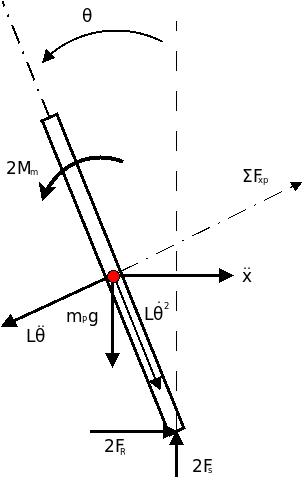
\includegraphics[width=5cm]{chasisPend}
\caption{Model šasi}
\label{fig:chasisPend}
\end{figure}

Na \figurename~\ref{fig:chasisPend} sú znázornené sily pôsobiace na šasi robota pri pohybe, pričom:

$\quad L$ = dĺžka šasi, meraná od stredu kolies

$\quad m_p$ = hmotnosť šasi

$\quad \theta$ = uhol náklonu šasi

$\quad \sum{F_{xp}}$ = súčet síl na virtuálnej osi xp

Význam ostatných veličín je zhodný s definíciami v predchádzajúcej časti. Je teda zjavné, že podľa očakávaní sú sily pôsobiace na podvozok premietnuté aj do modelu šasi. Z Newtonovho zákona po úprave dostaneme rovnicu v tvare:
\begin{equation}
2F_R = m_p \ddot{x} + m_p L \ddot{\theta} cos{\theta} - m_p L\dot{\theta}^2 sin\theta
\label{eq:horizontal}
\end{equation}

Táto rovnica predstavuje súčet síl na horizonálnej osi. Pre sily pôsobiace ne virtuálnej osi $F_px$, kolmo na šasi, platí vzťah \eqref{eq:perpend} a súčet momentov síl okolo ťažiska šasi je vyjadrený v \eqref{eq:around_center}.
\begin{equation}
2F_R cos\theta + 2F_S sin\theta - m_p g sin\theta - m_p L \ddot{\theta} = m_p \ddot{x}cos\theta
\label{eq:perpend}
\end{equation}
\begin{equation}
-2F_R L cos\theta - 2F_S L sin\theta - 2M_m = J_p \ddot{\theta}
\label{eq:around_center}
\end{equation}

Točivý moment motorov je potrebné linearizovať a teda:
\begin{equation}
2M_m = \dfrac{-2K_M K_e \dot{x}}{Rr} + \dfrac{2K_M U_m}{R}
\label{eq:linear_moment}
\end{equation}

Po dosadení \eqref{eq:linear_moment} do \eqref{eq:around_center} dostaneme \eqref{eq:subst}. Následne upravíme \eqref{eq:perpend} vynásobením $-L$ a prepísaním do tvaru \eqref{eq:rearanged}:
\begin{equation}
-2F_R L cos\theta - 2F_S L sin\theta = \dfrac{-2K_M K_e \dot{x}}{Rr} + \dfrac{2K_M U_m}{R} + J_p\ddot{\theta}
\label{eq:subst}
\end{equation}
\begin{equation}
-2F_R L cos\theta - 2F_S L sin\theta = -m_p g L sin\theta - m_p L^2 \ddot{\theta} - m_p L \ddot{x} cos\theta
\label{eq:rearanged}
\end{equation}

Odčítaním týchto dvoch rovníc dostávame:
\begin{equation}
\dfrac{-2K_M K_e \dot{x}}{Rr} + \dfrac{2K_M U_m}{R} + J_p\ddot{\theta} = -m_p g L sin\theta - m_p L^2\ddot{\theta} - m_p L \ddot{x} cos\theta
\label{eq:chasis}
\end{equation}

Z rovnice \eqref{eq:wheels} môžeme odstrániť člen $2F_R$ nahradením z \eqref{eq:horizontal}:
\begin{equation}
2(m_m - \dfrac{2J_k}{r^2}) \ddot{x} = \dfrac{-2K_M K_e}{R r^2}\dot{x}_k + \dfrac{2K_M}{Rr}U_m - m_p \ddot{x} - m_p L \ddot{\theta} cos\theta - m_p L \ddot{\theta}^2 sin\theta
\label{eq:wheels}
\end{equation}

Po vyjadrení \eqref{eq:chasis} a \eqref{eq:wheels} je potrebné rovnice linearizovať. Pri linearizácii predpokladáme, že uhol $\theta = 0 + \varphi$, kde $\varphi$ predstavuje malý uhol náklonu robota. Výsledkom linearizácie a následnej úpravy rovníc je výsledný model balansujúceho robota:
\begin{equation}
\begin{gathered}
\ddot{\varphi} = \dfrac{m_p L}{J_P L^2}\ddot{x} + \dfrac{2K_M K_e}{Rr(J_P + m_p L^2)}\dot{x} - \dfrac{2K_M}{R(J_P + m_p L^2)} U_m + \dfrac{m_p g L}{(J_P + m_p L^2)}\varphi
\\
\\
\ddot{x} = \dfrac{2K_M}{Rr(2m_k - \dfrac{2J_k}{r^2} + m_p)} U_m - \dfrac{2K_M K_e}{Rr^2(2m_k - \dfrac{2J_k}{r^2} + m_p) }\dot{x} + \dfrac{m_p L}{2m_k - \dfrac{2J_k}{r^2} + m_p}\ddot{\varphi}
\end{gathered}
\end{equation}

Relevantné parametre nami skonštruovaného robota sú zosumarizované v úvode kapitoly - \nameref{ch:chapFunc}.